\documentclass[11pt, a4paper]{article} 
\setlength{\oddsidemargin}{0.5cm}
\setlength{\evensidemargin}{0.5cm}
\setlength{\topmargin}{-1.6cm}
\setlength{\leftmargin}{0.5cm}
\setlength{\rightmargin}{0.5cm}
\setlength{\textheight}{24.00cm} 
\setlength{\textwidth}{15.00cm}
\parindent 0pt
\parskip 5pt
\pagestyle{plain}

\usepackage{pgfgantt} 


\title{Research Proposal}
\author{Marc Labouchardiere (23857377)}
\date{13 March 2026}

\newcommand{\namelistlabel}[1]{\mbox{#1}\hfil}
\newenvironment{namelist}[1]{%1
\begin{list}{}
    {
        \let\makelabel\namelistlabel
        \settowidth{\labelwidth}{#1}
        \setlength{\leftmargin}{1.1\labelwidth}
    }
  }{%1
\end{list}}

\usepackage[T1]{fontenc}
\usepackage{float}
\usepackage{tikz}
\usepackage{url}
\usetikzlibrary{arrows.meta, positioning, fit, backgrounds, calc}

% ── Colour palette ──────────────────────────────────────────
\definecolor{existblue}{HTML}{3B78A8}
\definecolor{existfill}{HTML}{D3E2EF}
\definecolor{proprust}{HTML}{C4572A}
\definecolor{propfill}{HTML}{F4DDD0}
\definecolor{stretchbdr}{HTML}{7B6928}
\definecolor{stretchfill}{HTML}{F2EACC}
\definecolor{grey}{HTML}{555555}

% ── Node styles ─────────────────────────────────────────────
\tikzset{
    base/.style={rectangle, rounded corners=3pt, align=center,
        minimum width=3.2cm, minimum height=1cm,
        line width=0.7pt, font=\small\sffamily\bfseries},
    existing/.style={base, draw=existblue, fill=existfill,
        text=existblue!85!black},
    proposed/.style={base, draw=proprust, fill=propfill,
        text=proprust!85!black},
    stretch/.style={base, draw=stretchbdr, fill=stretchfill,
        text=stretchbdr!85!black, densely dashed},
    arr/.style={-{Stealth[length=5pt]}, line width=0.6pt, color=grey},
    arrprop/.style={-{Stealth[length=5pt]}, line width=0.6pt,
        color=proprust},
    arrpropdash/.style={-{Stealth[length=5pt]}, line width=0.6pt,
        color=proprust, densely dashed},
    arrstr/.style={-{Stealth[length=5pt]}, line width=0.6pt,
        color=stretchbdr, densely dashed},
    lbl/.style={font=\scriptsize\sffamily, color=grey, align=center,
        fill=white, inner sep=2pt},
}



\begin{document}
\thispagestyle{empty}
\newpage
\setcounter{page}{1}
\maketitle

\begin{namelist}{xxxxxxxxxxxx}
\item[{\bf Title:}]
	Towards Reactive AI-Driven Moving Target Defence: Parameter Analysis and Adversarial Modelling in a Network Simulator
% \item[{\bf Author:}]
% 	Marc F. Labouchardiere
\item[{\bf Supervisor:}]
	Dr Jin B. Hong
\item[{\bf Degree:}]
	Bachelor of Advanced Computer Science (Honours)
\end{namelist}

\section{Introduction} 

\subsection{Moving Target Defence}

Moving Target Defence (MTD) is the deliberate creation of asymmetric uncertainty that redirects the cost advantage from the attacker to the defender \cite{jajodia2011}. The fundamental design principle for developing MTD techniques lies in the decisions for the following three questions: \textit{what to move, how to move, and when to move} \cite{cai2016}. Critically, there is a distinction between proactive MTD (reconfiguration at fixed intervals) and reactive MTD (triggered by specific events such as IDS alerts). This results in a fundamental trade-off. If the interval time is too large, the attacker has sufficient time to complete an attack before the next move. If the interval time is too small, the MTD triggers even when there is no attack on the system, wasting defence resources and degrading performance \cite{sengupta2020}. This is the core motivation for a reactive MTD that uses IDS feedback to make informed reconfiguration decisions rather than moving blindly.

Zhang (2023) \cite{zhang2023} extended the foundational \textit{MTDSim} simulator \cite{MTDSim} into \textit{MTDSimTime}, a Discrete-Event Simulation framework that integrates the time domain into the evaluation of combined MTD strategies. Zhang's evaluation demonstrates that network-shuffle-based techniques (IP Shuffle, Complete Topology Shuffle) consistently outperform diversity-based techniques by over 130\% on average. However, the work has several limitations that constrain the real-world scalability of its conclusions. First, the attacker model is notably shallow: only one of two originally available attack scenarios was implemented, and the adversary follows a fixed action sequence with no adaptive intelligence, representing the lowest common denominator of attacker sophistication. Second, the MTD operations module was reduced from seven techniques to four, and evaluation was limited to single and pairwise combinations only, leaving open the question of whether further combinations yield further gains. 

Tay (2024) \cite{tay2024} extended the \textit{MTDSimTime} framework by producing \textit{MTDShield}, a reinforcement learning module that uses Double Deep Q-Network (DDQN) to automate the selection and timing of MTD operations based on network security metrics. The system processes both static features and temporal metrics through separate neural network branches before fusing them to produce a set of five Q-values representing possible MTD actions. This work is a meaningful step towards reactive MTD deployment, moving beyond fixed-interval scheduling by basing defensive actions on the observed network state. However, \textit{MTDShield} has notable limitations. Most critically, some metrics used for decision making (such as Host Compromise Ratio or Mean Time to Compromise) are aggregate measures that assume the defender has complete and accurate knowledge of the network state. Further investigation of the input parameters driving MTD decision-making is needed to make the defence truly reactive.

Both works are constrained by aspects of the underlying simulation that remain underexplored. The attacker model lacks adaptive behaviour, the MTD action space remains artificially reduced from its original scope, and the input parameters driving the RL agent's decisions have not been systematically evaluated for their individual contribution to defensive outcomes. These elements require systematic investigation and strengthening as a precursor for further work.

\subsection{Intrusion Detection in Moving Target Defence}

MTD does not exist in isolation. An Intrusion Detection System (IDS) provides the observation channel through which defenders perceive attacker activity, while MTD provides the action space through which defenders alter the attack surface. The relationship is mutually reinforcing: MTD forces attackers into anomalous behaviours that IDS can more readily detect, while IDS provides the situational awareness needed for intelligent, event-driven reconfiguration rather than costly blind randomisation \cite{cho2020}. Previous works on this simulator \cite{zhang2023} characterised IDS and firewalls as static legacy mechanisms that MTD supersedes. This proposal adopts a more nuanced framing, treating IDS as an architectural complement to MTD. A consequence of this integration is that the defender never observes the true state of the network. The defender sees only noisy IDS alerts, subject to missed detections, false alarms, and variable latency \cite{khraisat2019}. Network defence under these conditions is fundamentally a problem of partial observability, formalised in the literature as a Partially Observable Markov Decision Process (POMDP) \cite{mcabee2021}. Current work on this simulator does not enforce any such constraint: the RL agent learns from network security metrics directly.

Tay \cite{tay2024} undertook a preliminary investigation into this gap through a sensitivity study that varied the proportion of attacker actions visible to the model during training, simulating the effect of imperfect detection. The study found that model performance degrades below 70\% detection visibility, with performance becoming uncorrelated with detection rate at lower sensitivities. However, this approach models IDS as a uniform random masking of attacker actions --- a single scalar parameter applied identically across all attack types. Replacing this simplified model with a realistic IDS observation layer is a key stretch goal of this work.

\subsection{Optimisation of MTD Operations}

Beyond the observation model, prior work has also optimised the reinforcement learning agent's configuration. Tay \cite{tay2024} evaluated DDQN hyperparameters and conducted ablation studies on the \textit{MTDShield} architecture, finding that removing either the static or temporal input module degraded performance by only 6--8\%. Dunstall (2025) \cite{dunstall2025} extended this through multi-objective optimisation using NSGA-II, introducing cost metrics such as downtime ratio and MTD action ratio alongside security metrics. However, both efforts inherit the full-observability assumptions, constrained action space, and simplified attacker model of the underlying simulator. This project includes systematic parameter exploration but treats it as a component of strengthening the simulation framework rather than an end in itself.

\section{Aim} 

This project aims to strengthen the \textit{MTDShield} simulation framework \cite{zhang2023, tay2024, dunstall2025} and systematically evaluate how the AI-MTD module's input parameters, observation configurations, and adversarial conditions affect its defensive performance. Prior work evaluated the RL agent under fixed configurations and a simplified attacker; this project addresses those constraints. Specifically, this project will:

\begin{itemize}
    \item \textbf{Develop a more sophisticated adversarial module} that exercises the AI-MTD agent beyond the capabilities of the existing baseline attacker, enabling non-trivial evaluation of defensive strategies.

    \item \textbf{Systematically explore AI-MTD input parameters and configurations} to identify which parameter regimes most meaningfully affect defensive outcomes.

    \item \textbf{Analyse and characterise the relationship between configuration choices and performance}, offering empirical insight into not only which settings improve outcomes but why.

    \item \textbf{(Stretch) Design and integrate an IDS observation module} that replaces the agent's current full-observability assumption with a realistic, partial-observation interface, and evaluate agent performance under degraded observation conditions.
    
\end{itemize}

\begin{figure}[H]
    \centering
    \resizebox{\textwidth}{!}{%
        \begin{tikzpicture}

% ================================================================
%  SIMULATION ENVIRONMENT
% ================================================================

\node[proposed] (attacker) at (0, 4.2) {Enhanced\\Attacker Module};
\node[existing] (network)  at (4.5, 4.2) {Network};
\node[existing] (mtd)      at (2.25, 1.2) {MTD\\Operations};

\draw[arr] (attacker) --
    node[lbl, above] {Compromise Hosts} (network);
\draw[arr] (mtd.north west) --
    node[lbl, left, pos=0.5] {Interrupt\\[-2pt]Actions} (attacker.south);
\draw[arr] (mtd.north east) --
    node[lbl, right, pos=0.5] {Reconfigure\\[-2pt]Network} (network.south);

\begin{scope}[on background layer]
    \node[draw=grey, densely dashed, rounded corners=6pt,
          line width=0.9pt, inner xsep=16pt, inner ysep=16pt,
          fit=(attacker)(network)(mtd),
          label={[font=\small\sffamily\bfseries, text=grey,
                  anchor=north west, xshift=5pt, yshift=-5pt
                 ]north west:Simulation Environment}
         ] (simbox) {};
\end{scope}

% ================================================================
%  IDS MODULE (stretch)
% ================================================================

\node[stretch, minimum width=2.6cm] (ids) at (8.5, 4.2) {IDS\\Module};

% ================================================================
%  RL DEFENDER AGENT
% ================================================================

% Input column
\node[existing, minimum width=3.2cm] (existobs) at (12.5, 5.2)
    {Existing Observation\\Pipeline};
\node[stretch, minimum width=3.2cm] (idsalert) at (12.5, 3.2)
    {IDS Alert\\Processing};
\node[proposed, minimum width=3.2cm] (params) at (12.5, 1.2)
    {Parameter \&\\Configuration Inputs};

% Processing column
\node[existing, minimum width=3.2cm] (state) at (17.2, 3.2)
    {State\\Representation};
\node[existing, minimum width=3.2cm] (qnet)  at (17.2, 1.2)
    {Q-Network\\Output Layer};
\node[existing, minimum width=3.2cm] (action) at (17.2, -0.6)
    {Action\\Selection};

% Inputs → State (clear horizontal fan)
\draw[arr] (existobs.east) --
    node[lbl, above, pos=0.45] {Static \&\\[-2pt]Temporal Features}
    (state.north west);
\draw[arrstr] (idsalert.east) --
    node[lbl, above, pos=0.45] {Alert\\[-2pt]Features}
    (state.west);
\draw[arrprop] (params.east) --
    node[lbl, below, pos=0.45] {Experimental\\[-2pt]Configurations}
    (state.south west);

% Processing pipeline
\draw[arr] (state.south) --
    node[lbl, right, pos=0.5] {Processed Features}
    (qnet.north);
\draw[arr] (qnet.south) --
    node[lbl, right, pos=0.5] {Q-Values}
    (action.north);

\begin{scope}[on background layer]
    \node[draw=grey, densely dashed, rounded corners=6pt,
          line width=0.9pt, inner xsep=16pt, inner ysep=16pt,
          fit=(existobs)(idsalert)(params)(state)(qnet)(action),
          label={[font=\small\sffamily\bfseries, text=grey,
                  anchor=north west, xshift=5pt, yshift=-5pt
                 ]north west:RL Defender Agent}
         ] (rlbox) {};
\end{scope}

% ================================================================
%  CROSS-REGION ARROWS
% ================================================================

% 1. Network → Existing Observation Pipeline (routed above)
\draw[arr]
    (network.north) -- ++(0, 2.8)
    -| (existobs.north);
\node[lbl] at (8.5, 7.0) {Network Security Metrics};

% 2. Network → IDS (horizontal)
\draw[arrstr] (network.east) --
    node[lbl, above, pos=0.5] {Network Events}
    (ids.west);

% 3. IDS → IDS Alert Processing (diagonal)
\draw[arrstr] (ids.east) --
    node[lbl, above, sloped, pos=0.45] {Alerts}
    (idsalert.west);

% 4. Simulation → Parameters (researcher investigation)
\draw[arrpropdash]
    (simbox.east |- params) --
    node[lbl, above, pos=0.5] {Empirical Investigation}
    (params.west);

% ================================================================
%  OUTPUT PATHS (fork well below RL box boundary)
% ================================================================

% Fork point — clearly below the RL agent boundary
\coordinate (fork) at (17.2, -2.2);
\draw[color=grey, line width=0.6pt] (action.south) -- (fork);
\fill[grey] (fork) circle (1.8pt);

% 5. Fork → MTD Operations (grey, loops back along the bottom)
\draw[arr]
    (fork) -- ++(0, -0.8)
    -| (mtd.south);
\node[lbl] at (9.5, -3.6) {Selected MTD Action};

% 6. Fork → Analysis & Evaluation (orange dashed, branches left)
\node[proposed, minimum width=3.2cm] (analysis) at (8.5, -4.6)
    {Analysis \&\\Evaluation};

\draw[arrpropdash]
    (fork) -|
    node[lbl, text=proprust!80!black, above, pos=0.25]
        {Performance Metrics}
    (analysis.north);

% ================================================================
%  LEGEND (bottom-left)
% ================================================================

\node[existing, minimum width=1.6cm, minimum height=0.4cm,
      font=\scriptsize\sffamily\bfseries]
      (leg1) at (-1.6, -3.6) {};
\node[right=3pt of leg1, font=\scriptsize\sffamily, text=grey]
      {Existing component};

\node[proposed, minimum width=1.6cm, minimum height=0.4cm,
      font=\scriptsize\sffamily\bfseries, below=5pt of leg1.south west,
      anchor=north west]
      (leg2) {};
\node[right=3pt of leg2, font=\scriptsize\sffamily, text=grey]
      {Proposed contribution (core)};

\node[stretch, minimum width=1.6cm, minimum height=0.4cm,
      font=\scriptsize\sffamily\bfseries, below=5pt of leg2.south west,
      anchor=north west]
      (leg3) {};
\node[right=3pt of leg3, font=\scriptsize\sffamily, text=grey]
      {Proposed contribution (stretch)};

\end{tikzpicture}
    }
    \caption{Overview of proposed contributions to the simulation architecture.}
    \label{fig:proposed-contributions}
\end{figure}

\section{Method}

This section outlines the approach for achieving each aim identified above, broken into sequential and overlapping phases. A consolidated timeline is presented in Section~\ref{subsec:timeline}.

\subsection{Codebase Comprehension and Baseline Establishment}\label{subsec:baseline}

A prerequisite to any experimental contribution is a thorough
understanding of the existing \textit{MTDShield} codebase and its
antecedents \cite{zhang2023, tay2024}. This phase, conducted in parallel
with the literature review (March--April 2026), involves auditing the
simulator architecture, reproducing key results from prior work to
establish baseline performance figures, and documenting the codebase to
support future extension. Baseline reproduction serves as the completion
criterion: the phase is complete when prior results have been independently
verified within an acceptable margin.

\subsection{Adversarial Model Enhancement}

The existing attacker follows a fixed action sequence with no adaptive
behaviour, and only one of two originally available attack objectives was
implemented \cite{zhang2023}. This phase strengthens the adversarial module
by first reintegrating the second attack objective, then introducing more
sophisticated attack behaviours informed by mapping the simulator's action
space to the MITRE ATT\&CK framework to identify coverage gaps. New attack
scenarios will implement multi-stage kill chains combining reconnaissance,
lateral movement, and privilege escalation, calibrated so that the current
AI-MTD policy exhibits measurable degradation relative to the baselines
from Section~\ref{subsec:baseline}. This phase is estimated at
approximately two months (May--June 2026).

\subsection{Parameter Exploration and Evaluation}\label{subsec:param}

With an enhanced attacker in place, this phase systematically varies the
AI-MTD module's inputs and configurations across three categories:
observation features, action-space configuration, and training
hyperparameters (reward shaping, discount factor, exploration schedule).
For each category, individual parameters will be varied against a held
baseline (ablation studies), followed by interaction effects between
promising combinations. Where parameter changes produce significant
performance differences, further analysis will seek to explain
\textit{why} --- for example, examining which observation features
correlate most strongly with effective action selection. This phase runs
concurrently with the later stages of adversarial enhancement (late
May--late July 2026).

\subsection{IDS Integration (Stretch Goal)}

This phase is contingent on satisfactory progress in the preceding phases
and is scoped as a proof of concept. The objective is to replace the RL
agent's current full-observability assumption with an IDS module that
intercepts simulated attacker events and produces alerts with configurable
detection probability, false positive rate, and detection latency.
The agent's observation space would be rewired to receive these alerts
rather than ground-truth network state, and retrained under
partial-observability conditions. The parameter exploration from
Section~\ref{subsec:param} would then be extended to evaluate performance
as IDS fidelity is varied, building on Tay's preliminary sensitivity
analysis \cite{tay2024}. If reached, this phase would occupy approximately
August--September 2026.

\subsection{Timeline}\label{subsec:timeline}

\begin{figure}[H]
\centering
\resizebox{\textwidth}{!}{%
\begin{ganttchart}[
    x unit=0.55cm,
    y unit title=0.5cm,
    y unit chart=0.55cm,
    title height=1,
    vgrid={*1{dotted}},
    hgrid,
    bar height=0.45,
    bar top shift=0.275,
    group/.append style={draw=black, fill=black!15},
    group label font=\footnotesize\bfseries,
    bar label font=\footnotesize,
    milestone label font=\footnotesize\bfseries,
    title label font=\footnotesize\bfseries,
    link/.style={-latex, thick, rounded corners=2pt},
    link bulge=1.5,
    today=3,
    today label=Today,
    today label font=\scriptsize\itshape,
    today rule/.style={draw=red!60, ultra thick, dashed},
]{1}{33}

    % Title: weeks from early March to mid October 2026
    % ~33 weeks: Mar 2 -> Oct 16
    \gantttitle{2026}{33} \\
    \gantttitle{March}{4}
    \gantttitle{April}{5}
    \gantttitle{May}{4}
    \gantttitle{June}{4}
    \gantttitle{July}{5}
    \gantttitle{August}{4}
    \gantttitle{Sept}{5}
    \gantttitle{Oct}{2} \\

    % ── Phase 1: Literature Review & Codebase ──────────────
    \ganttgroup{Phase 1: Foundations}{1}{12} \\

    \ganttbar[bar/.append style={fill=blue!25}]
        {Literature review}{1}{11} \\

    \ganttbar[bar/.append style={fill=blue!25}]
        {Codebase audit \& documentation}{1}{9} \\

    \ganttbar[bar/.append style={fill=blue!25}]
        {Baseline reproduction}{5}{9} \\

    \ganttbar[bar/.append style={fill=blue!25}]
        {RL / ML self-study}{1}{9} \\

    \ganttmilestone[milestone/.append style={fill=red!70}]
        {Literature review due (22 May)}{12} \\

    % ── Phase 2: Adversarial Enhancement ───────────────────
    \ganttgroup{Phase 2: Adversarial Enhancement}{9}{18} \\

    \ganttbar[bar/.append style={fill=orange!30}]
        {Reintegrate 2nd attack objective}{9}{12} \\

    \ganttbar[bar/.append style={fill=orange!30}]
        {ATT\&CK mapping \& coverage analysis}{11}{14} \\

    \ganttbar[bar/.append style={fill=orange!30}]
        {Multi-stage attack implementation}{13}{18} \\

    \ganttbar[bar/.append style={fill=orange!30}]
        {Validation against baselines}{17}{18} \\

    % ── Phase 3: Parameter Exploration ─────────────────────
    \ganttgroup{Phase 3: Parameter Exploration}{12}{22} \\

    \ganttbar[bar/.append style={fill=green!25}]
        {Ablation studies (observation, action, hyperparams)}{12}{19} \\

    \ganttbar[bar/.append style={fill=green!25}]
        {Interaction / combination experiments}{18}{22} \\

    \ganttbar[bar/.append style={fill=green!25}]
        {Analysis \& characterisation}{20}{24} \\

    % ── Phase 4: IDS Integration (Stretch) ─────────────────
    \ganttgroup[group/.append style={fill=black!8, draw=black!50, densely dashed}]
        {Phase 4: IDS Integration (Stretch)}{22}{31} \\

    \ganttbar[bar/.append style={fill=yellow!25, densely dashed}]
        {IDS module design \& calibration}{22}{26} \\

    \ganttbar[bar/.append style={fill=yellow!25, densely dashed}]
        {RL agent rewiring \& retraining}{26}{29} \\

    \ganttbar[bar/.append style={fill=yellow!25, densely dashed}]
        {IDS noise / fidelity experiments}{28}{31} \\

    % ── Phase 5: Cost Metrics (Stretch) ────────────────────
    \ganttbar[bar/.append style={fill=yellow!10, densely dashed}]
        {Cost metric integration (Stretch)}{26}{31} \\

    % ── Writing & Submission ───────────────────────────────
    \ganttgroup{Dissertation \& Seminar}{1}{33} \\

    \ganttbar[bar/.append style={fill=gray!20}]
        {Incremental writing}{5}{28} \\

    \ganttbar[bar/.append style={fill=gray!40}]
        {Seminar preparation}{27}{31} \\

    \ganttbar[bar/.append style={fill=gray!40}]
        {Final dissertation consolidation}{28}{33} \\

    \ganttmilestone[milestone/.append style={fill=red!70}]
        {Seminar (2 Oct)}{31} \\

    \ganttmilestone[milestone/.append style={fill=red!70}]
        {Dissertation due (16 Oct)}{33} \\

    % ── Dependencies ───────────────────────────────────────
    % Baseline reproduction -> Adversarial enhancement
    \ganttlink[link/.style={-latex, thick, color=blue!50}]{elem3}{elem7}
    % Baseline reproduction -> Parameter exploration (ablation)
    \ganttlink[link/.style={-latex, thick, color=blue!50}]{elem3}{elem12}
    % Lit review milestone -> ATT&CK mapping
    \ganttlink[link/.style={-latex, thick, color=red!50}]{elem5}{elem8}
    % Reintegrate attacker -> multi-stage attacks
    \ganttlink[link/.style={-latex, thick, color=orange!50}]{elem7}{elem9}
    % Multi-stage validation -> interaction experiments
    \ganttlink[link/.style={-latex, thick, color=orange!50}]{elem10}{elem13}
    % Analysis -> IDS module design
    \ganttlink[link/.style={-latex, thick, color=green!50, densely dashed}]{elem14}{elem16}
    % IDS module -> RL rewiring
    \ganttlink[link/.style={-latex, thick, color=yellow!70!black, densely dashed}]{elem16}{elem17}
    % RL rewiring -> IDS experiments
    \ganttlink[link/.style={-latex, thick, color=yellow!70!black, densely dashed}]{elem17}{elem18}

\end{ganttchart}
}%
\caption{Project timeline. Dashed elements
indicate stretch goals.}
\label{fig:gantt}
\end{figure}
\section{Project Requirements}

The project will be conducted in Python~3, expanding on the
\textit{MTDShield} \cite{tay2024} framework and its dependencies. All
prior codebases are publicly available on GitHub. Training of
reinforcement learning models will be performed on commodity hardware;
no specialised GPU infrastructure is anticipated. The simulator
generates synthetic network data and does not involve human subjects,
personal data, or external datasets; no ethics approval is required.
Writing and code production will be assisted through the use of
Claude Opus 4.6. No IP or access restrictions have been identified.

\begin{thebibliography}{99}

\bibitem{jajodia2011}
S. Jajodia, A.~K. Ghosh, V. Swarup, C. Wang, and X.~S. Wang, Eds.,
\textit{Moving Target Defense: Creating Asymmetric Uncertainty for Cyber
Threats}, ser. Advances in Information Security, vol.~54.\hskip 1em
New York, NY, USA: Springer, 2011.

\bibitem{cai2016}
G.-l. Cai, B.-s. Wang, W. Hu, and T.-z. Wang,
``Moving target defense: State of the art and characteristics,''
\textit{Frontiers of Information Technology \& Electronic Engineering},
vol.~17, no.~11, pp.~1122--1153, Nov. 2016.

\bibitem{sengupta2020}
S. Sengupta, A. Chowdhary, A. Sabur, A. Alshamrani, D. Huang,
and S. Kambhampati,
``A survey of moving target defenses for network security,''
\textit{IEEE Communications Surveys \& Tutorials}, vol.~22, no.~3,
pp.~1909--1941, Jul. 2020.

\bibitem{zhang2023}
W. Zhang, ``Evaluating multiple moving target defence in the time domain,''
Master's thesis, School of Engineering, The University of Western Australia,
2023.

\bibitem{MTDSim}
A. Brown, ``MTDSim,'' GitHub repository, School of Engineering,
The University of Western Australia, 2021. [Online]. Available:
\url{https://github.com/Ccamm/MTDSim}

\bibitem{tay2024}
J.~K. Tay, ``Using artificial intelligence to automate the deployment of
moving target defence operations,''
Master's thesis, School of Engineering, The University of Western Australia,
2024.

\bibitem{cho2020}
J.-H. Cho, D.~P. Sharma, H. Alavizadeh, S. Yoon, N. Ben-Asher,
T.~J. Moore, D.~S. Kim, H. Lim, and F.~F. Nelson,
``Toward proactive, adaptive defense: A survey on moving target defense,''
\textit{IEEE Communications Surveys \& Tutorials}, vol.~22, no.~1,
pp.~709--745, 2020.

\bibitem{khraisat2019}
A. Khraisat, I. Gondal, P. Vamplew, and J. Kamruzzaman,
``Survey of intrusion detection systems: Techniques, datasets and
challenges,''
\textit{Cybersecurity}, vol.~2, no.~1, art.~20, 2019.

\bibitem{mcabee2021}
A.~S.~M. McAbee, M. Tummala, and J.~C. McEachen,
``The use of partially observable Markov decision processes to optimally
implement moving target defense,''
in \textit{Proc. 54th Hawaii Int. Conf. Syst. Sci. (HICSS)}, 2021,
pp.~1--10.

\bibitem{dunstall2025}
K. Dunstall, ``Multi-objective optimisation of artificial intelligence
automated deployment of moving target defence,''
Honours thesis, School of Engineering, The University of Western Australia,
2025.

\end{thebibliography}

\end{document}
